\pgfsetplotmarksize{0pt}
\begin{figure}
 \centering
 \caption{\label{fl_conv9}UflLib/Euclid/1911EuclS.txt},
 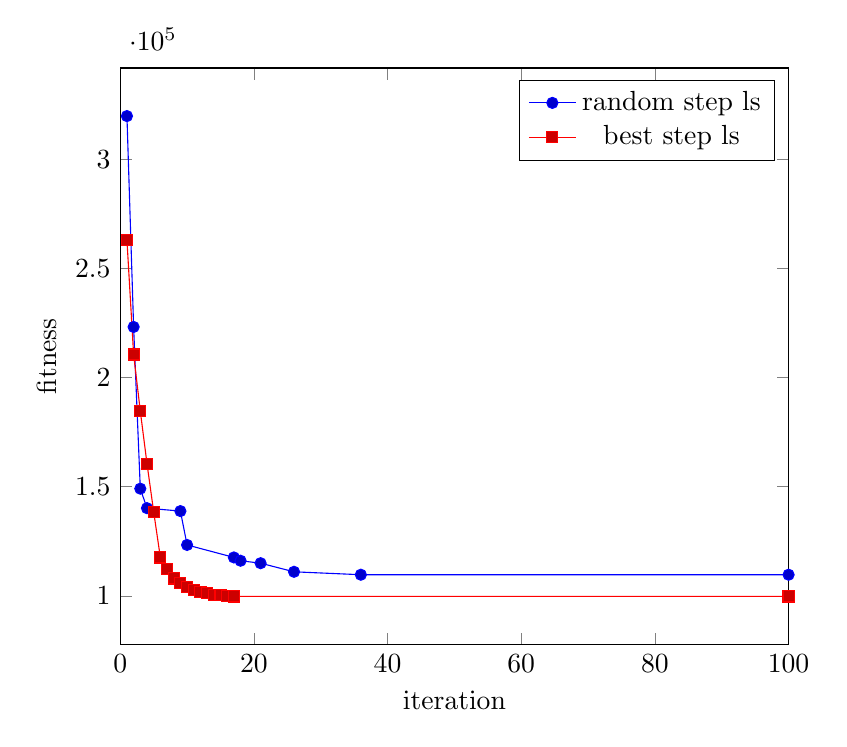
\begin{tikzpicture}
 \begin{axis}[
   width=0.7\textwidth,
   scale only axis,
   xlabel=iteration,
   ylabel=fitness,
   xmin=0,xmax=100,
   domain=0:100]
   \addplot coordinates {
     (0,inf)
     (1,319703)
     (2,223140)
     (3,149082)
     (4,140157)
     (9,138812)
     (10,123310)
     (17,117598)
     (18,116077)
     (21,114951)
     (26,111010)
     (36,109675)
     (100,109675)
   };
   \addlegendentry{random step ls}
   \addplot coordinates {
     (0,inf)
     (1,262903)
     (2,210520)
     (3,184577)
     (4,160564)
     (5,138503)
     (6,117595)
     (7,112187)
     (8,107971)
     (9,105713)
     (10,103929)
     (11,102615)
     (12,101895)
     (13,101144)
     (14,100500)
     (15,100357)
     (16,99819)
     (17,99729)
     (100,99729)
   };
   \addlegendentry{best step ls}
 \end{axis}
 \end{tikzpicture}
\end{figure}
